\section{Final Implementation}

%----------------------------------------------------------------------------------------
%	Subsection
%----------------------------------------------------------------------------------------

\begin{frame}
\frametitle{Improvements on previous work (word recognition)}
\begin{enumerate}
\item Coefficients that intensively require floating-point computations are precomputed. (Hamming window, Mel-bank filter gain and discrete cosine transform)
\item Frame energy is calculated in fixed-point arithmetic.
\item Sparse matrices are stored in ingeniously designed structures. Meaningless multiplications with zeros are illuminated. (Mel bank filter gain, inversed variance matrices and transition matrices)
\item Symmetry is sufficiently taken in to consideration. (FFT of real sequence and discrete cosine transform)
\end{enumerate}
\end{frame}

%----------------------------------------------------------------------------------------
%	Subsection
%----------------------------------------------------------------------------------------

\begin{frame}
\frametitle{Performance on DSP Board}
We randomly test the word recognition system on DSP and compare the outcomes computed by DSP and MATLAB for 23 times.
\begin{itemize}
	\item for dataset $n$ ($n = 1, 2, \dots, 23$) and word $k$ ($k = 1, 2, \dots, 27$)
	\item $p_{MATLAB}[n, k]$ denotes the probability (natural-log scale) computed by MATLAB
	\item $p_{DSP}[n, k]$ denotes the probability (natural-log scale) computed by DSP
\end{itemize}

The \textit{relative error} of word $k$ in dataset $n$
\begin{equation}
\varepsilon[n, k] = \frac{p_{DSP}[n, k] - p_{MATLAB}[n, k]}{p_{MATLAB}[n, k]}
\end{equation}
The \textit{Root Mean Square Error} of dataset $n$
\begin{equation}
\epsilon_{RMSE}[n] = \sqrt{\frac{1}{27} \sum_{k = 1}^{27} (\varepsilon[n, k])^2}
\end{equation}
\end{frame}

%--------------------------------------------
%--------------------------------------------

\begin{frame}
Absolute relative error $|\varepsilon[n, k]|$ ranges from $1 \times 10^{-6}$ to $9 \times 10^{-3}$ and dataset 1 has the largest deviation (\textcolor{navy_matlab}{navy solid line}).

\begin{figure}[H]
\centering
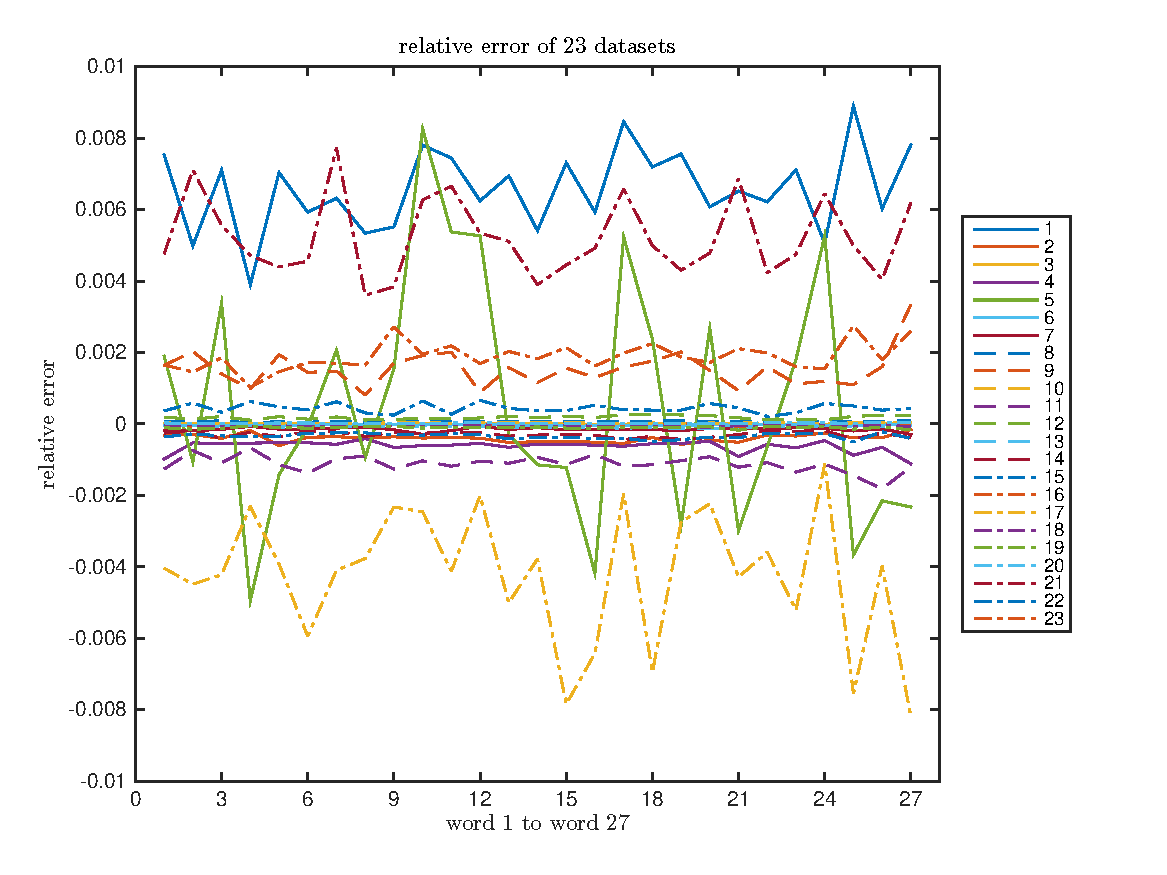
\includegraphics[width=3in, trim={0 0.6cm 0 0.6cm}, clip]{ang/relative_error}
\end{figure}
\end{frame}

%--------------------------------------------
%--------------------------------------------

\begin{frame}
Dataset 1 has the largest root mean square error $\epsilon_{RMSE}[n]$ consistently.

\begin{figure}[H]
\centering
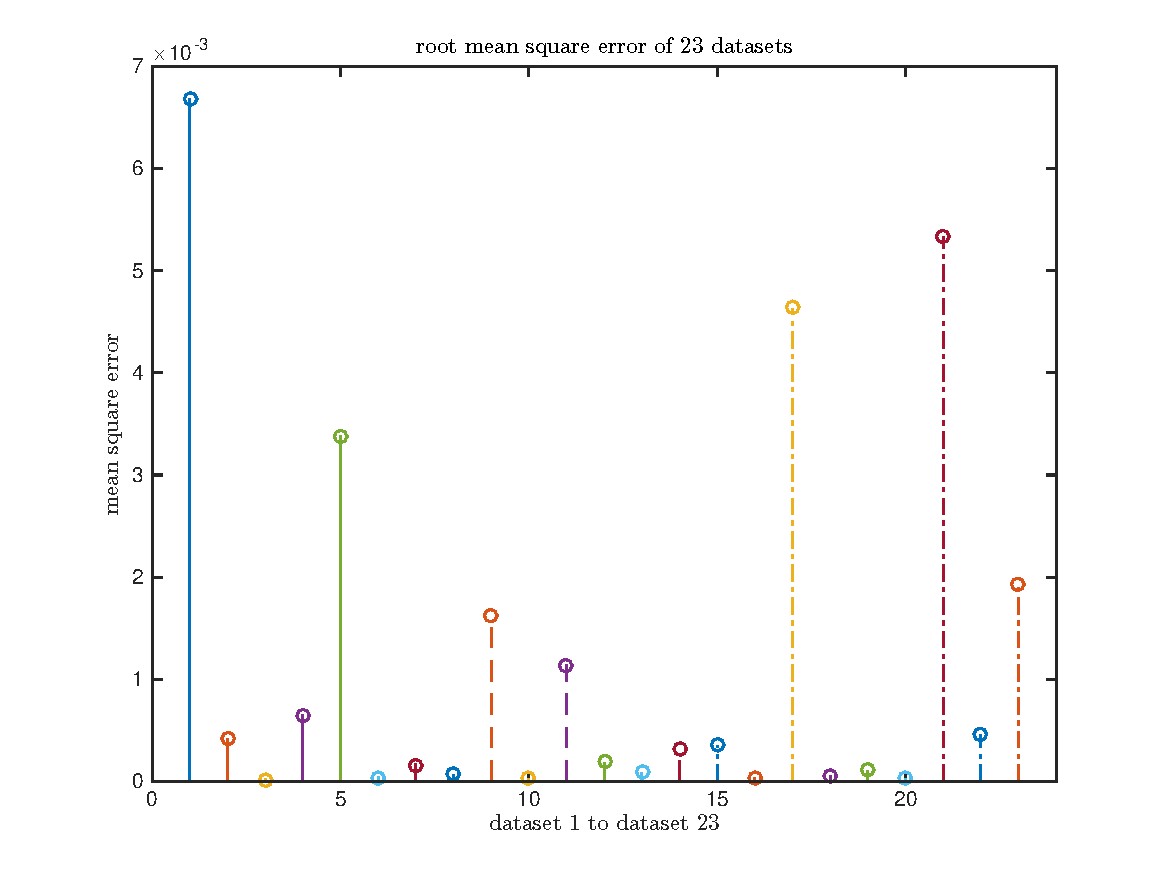
\includegraphics[width=3in, trim={0 0.6cm 0 0.6cm}, clip]{ang/root_mean_square_error}
\caption{the root mean square error $\epsilon_{RMSE}[n]$ of each dataset $n$}
\end{figure}
\end{frame}

%--------------------------------------------
%--------------------------------------------

\begin{frame}
\begin{itemize}
\item The computation error has no influence on recognition result.
\item Take the worst case (dataset 1) as an example.
\item Probabilities of 27 words computed by MATLAB (\textcolor{navy_matlab}{navy circle $\circ$}) and DSP (\textcolor{orange_matlab}{orange cross $\times$}) are so close to each other. (much less than the differences between probabilities.)
\end{itemize}

\begin{figure}[H]
\centering
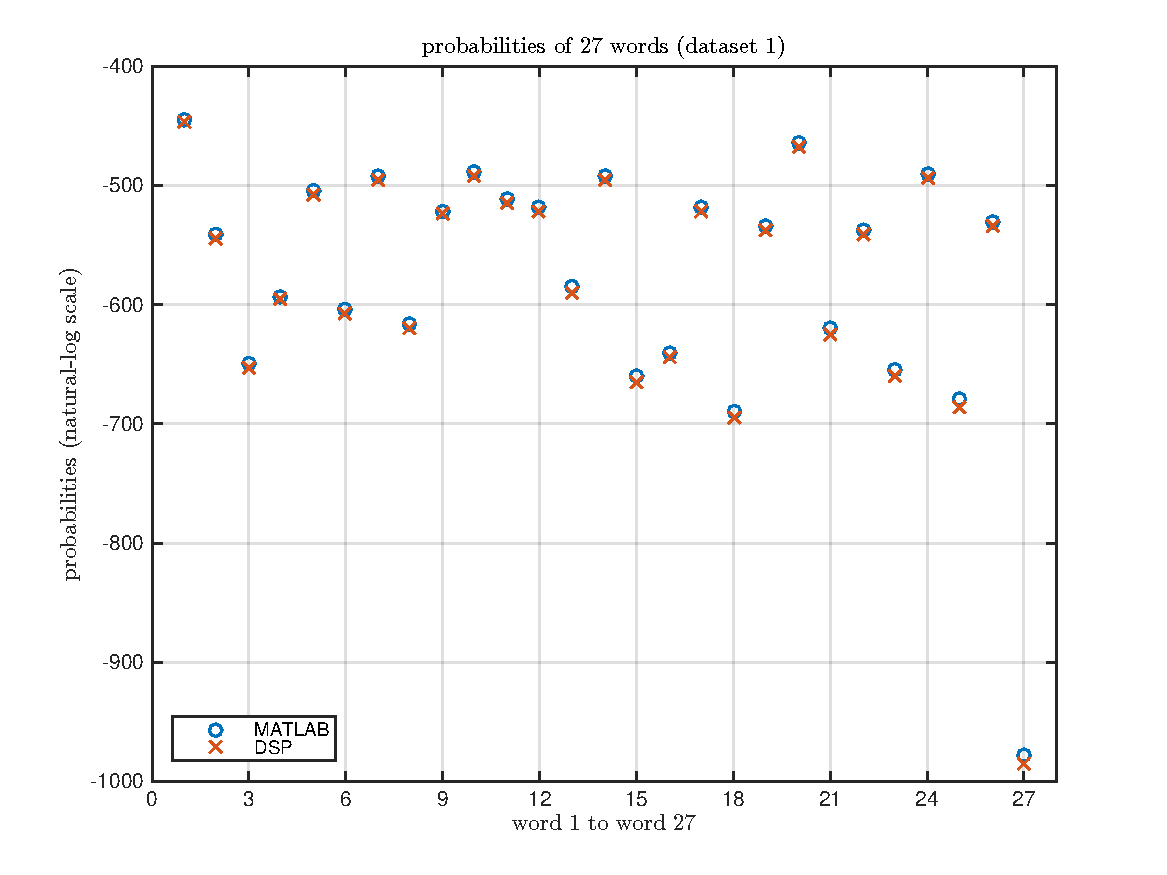
\includegraphics[width=3in, trim={0 0.6cm 0 0.6cm}, clip]{ang/word_probabilities}
\end{figure}
\end{frame}

%--------------------------------------------
%--------------------------------------------

\begin{frame}
Feature Extraction \& Recognition
\begin{itemize}
\item The average processing time of these 23 datasets is 95.8 ms.
\item The maximal processing time is 150 ms.
\end{itemize}

\begin{figure}[H]
\centering
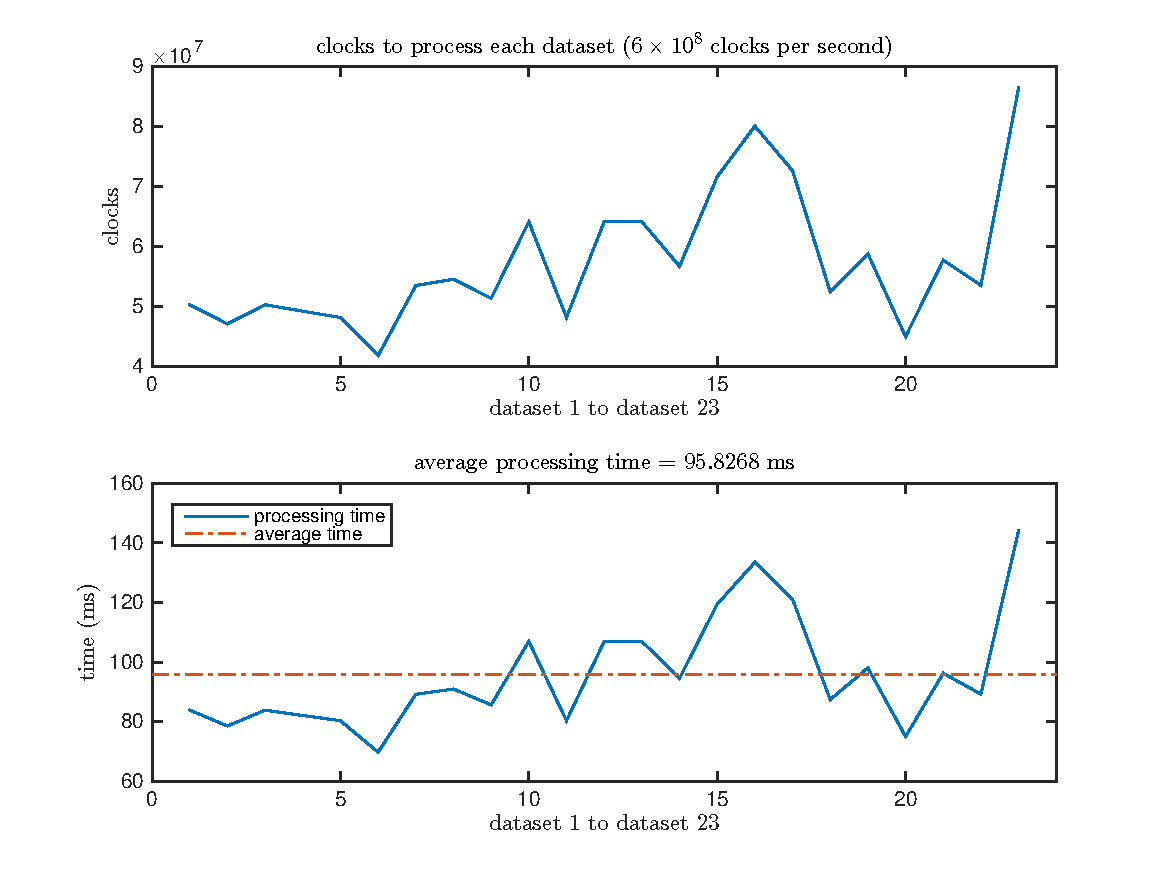
\includegraphics[width=3in, trim={0 0.6cm 0 0.6cm}, clip]{ang/processing_time}
\end{figure}
\end{frame}

%----------------------------------------------------------------------------------------
%	Subsection
%----------------------------------------------------------------------------------------

\begin{frame}
\frametitle{Final system implemented on DSP board}
\begin{itemize}
	\item Adaptive noise cancellation based on Least Mean Square Algorithm
	\item Real-time recognition of spoken words
	\item Result indication via a five-LED array
		\begin{itemize}
		\item \LED\offLED\offLED\offLED\offLED\onLED $\longrightarrow$ $(00001)_2 = 1$ $\longrightarrow$ word \textit{one}
		\item \LED\offLED\onLED\onLED\onLED\onLED $\longrightarrow$ $(01111)_2 = 15$ $\longrightarrow$ word \textit{fifteen}
		\item \LED\onLED\offLED\onLED\offLED\onLED $\longrightarrow$ $(10101)_2 = 21$ $\longrightarrow$ word \textit{zero}
		\item \LED\offLED\offLED\offLED\offLED\offLED $\longrightarrow$ $(00000)_2 = 0$ $\longrightarrow$ error
		\end{itemize}
	\item YouTube controller
\end{itemize}
\end{frame}
